\section{Byttehandel}

En af de primærer funktioner for projektet er, at brugere skal kunne anmode om en byttehandel, have mulighed for at kontakte hinanden, bytte og til sidst give hinanden en anmeldelse. 
Før man har mulighed for at bytte, kræves det at man har en bruger, som har oprettet mindst en annonce. En annonce kan kun byttes en gang. Det fungerer sådan, at person1 sender en bytteanmodning til person2. Person2 kan derved godkende eller afvise anmodningen se figur \ref{fig:BytteanmodningEks}. Ved godkendelse bliver anmodning sendt tilbage til person1, det skyldes at personen kan have ændret mening. Person1 kan derfor også godkende eller afvise. Ved godkendelse bliver byttehandlen færdiggjort, og både person 1 og 2 får byttehandlen ind i deres byttehistorik.

\begin{figure}[H]
	\centering
	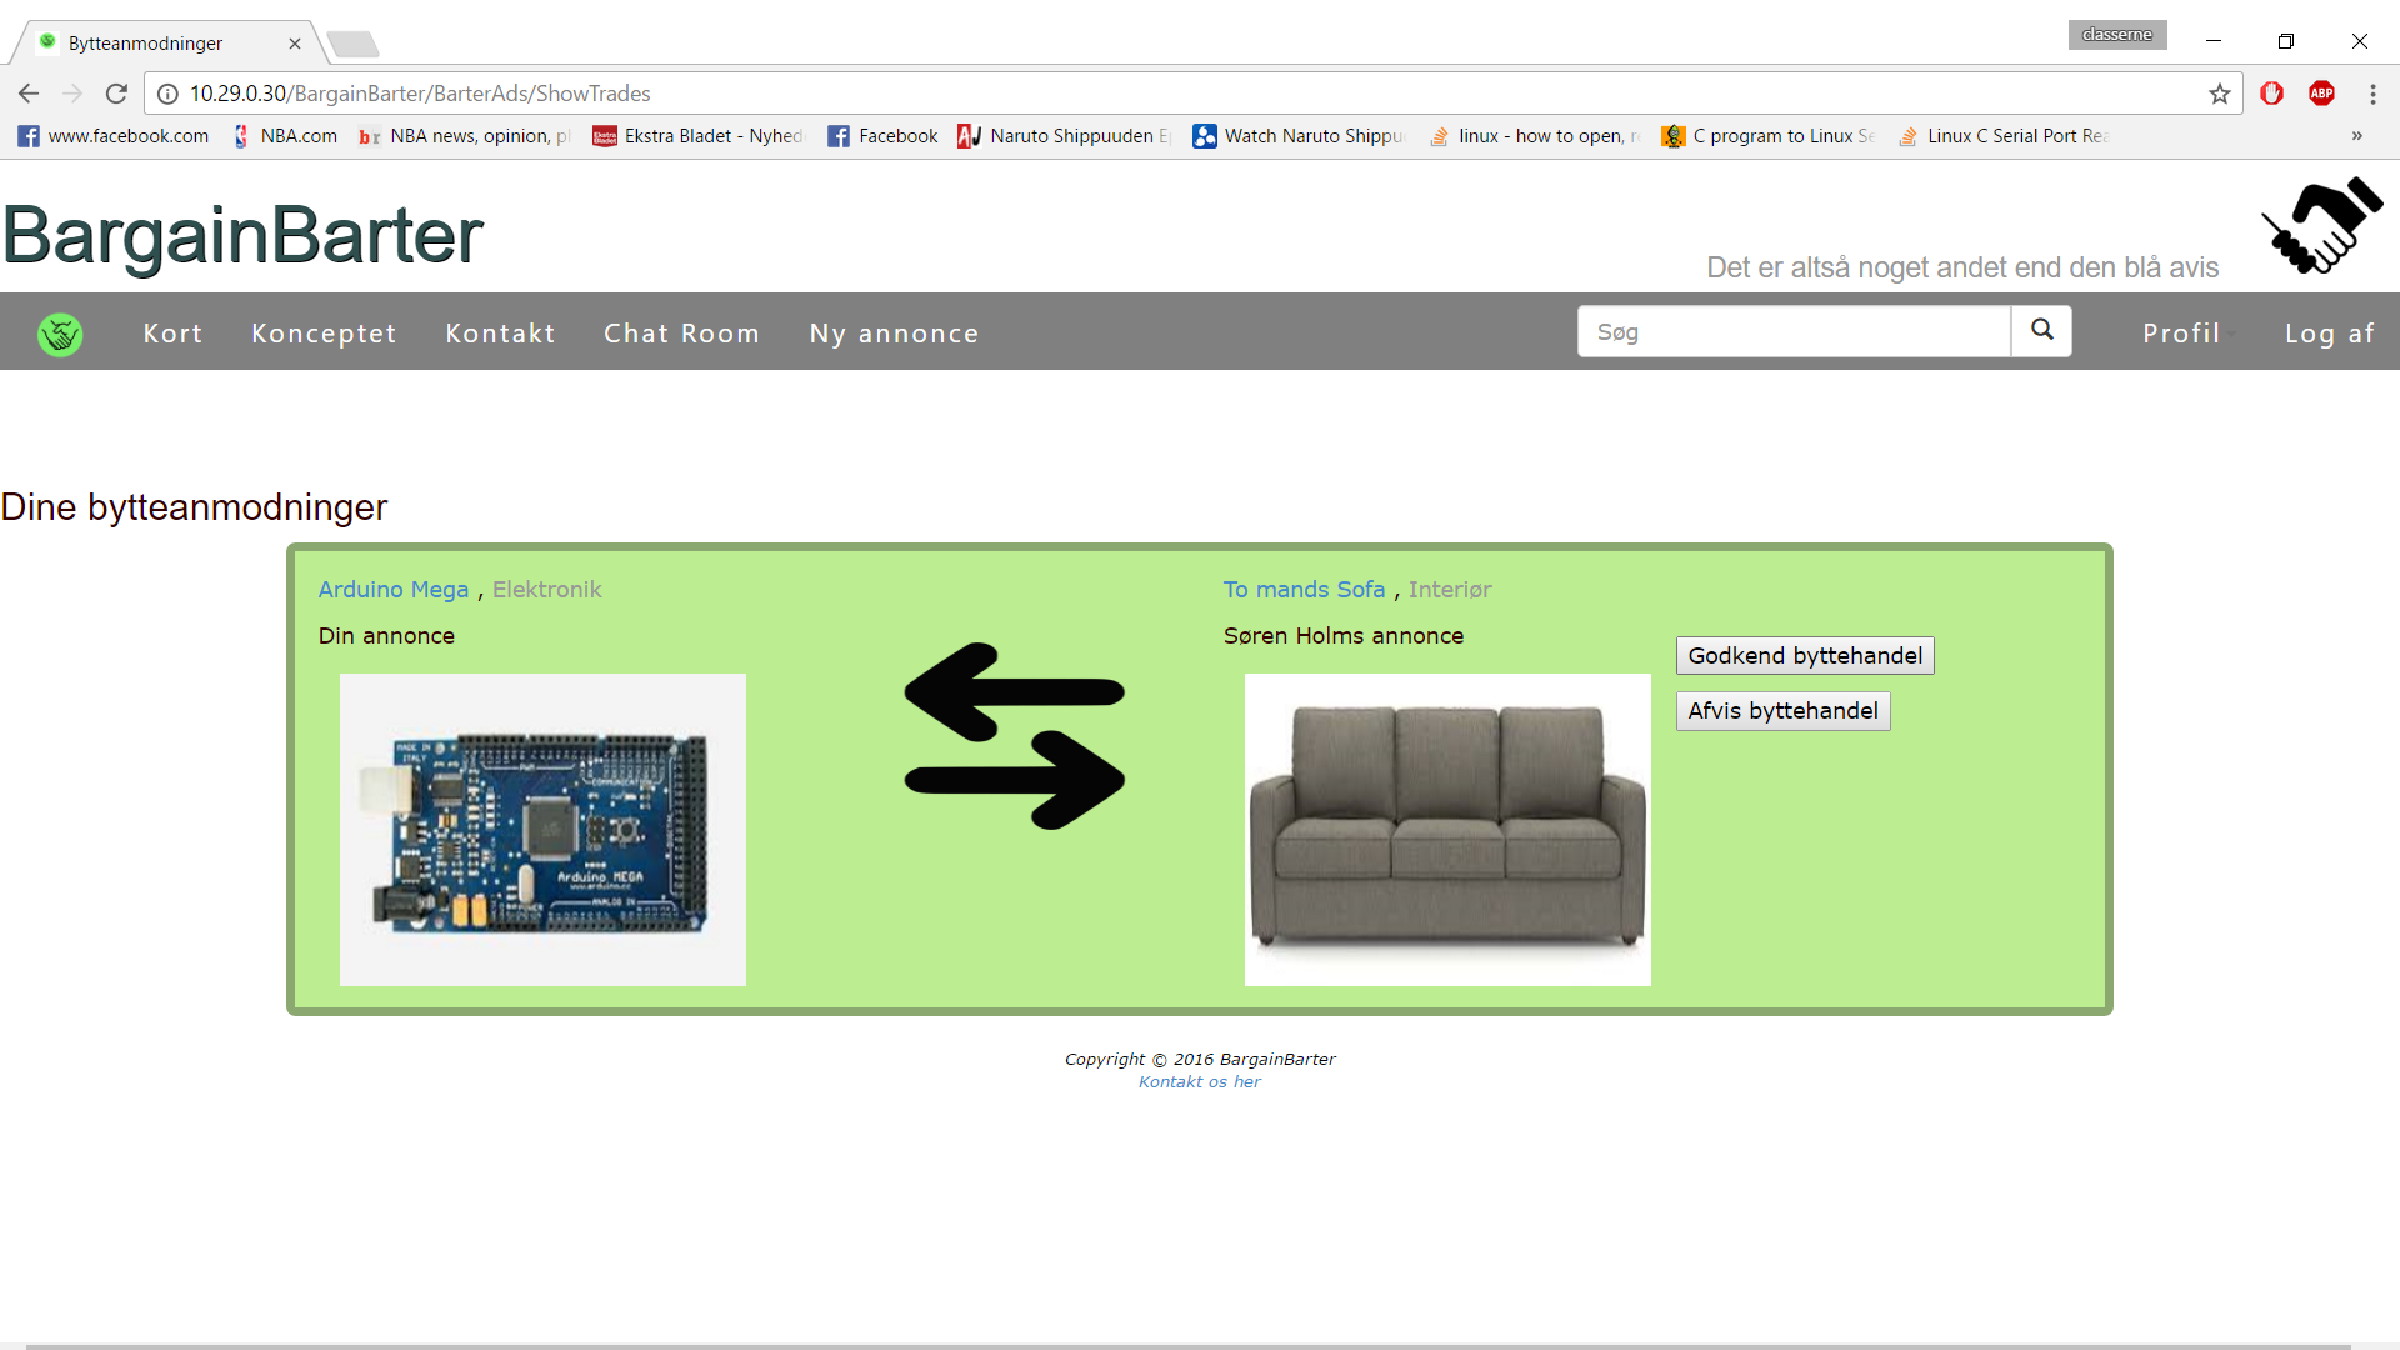
\includegraphics
	[width=165mm]
	{figures/Bytteanmodning.pdf}
	\caption{View for bytteanmodninger}
	\label{fig:BytteanmodningEks}
\end{figure}

Det er nu muligt for de 2 personer, at give hinanden en anmeldelse med kommentar og rating, alt efter hvordan handlen forløb.
De 2 annoncer er nu kun synlige i byttehistorikken, og kan ikke tilgås i andre byttehandler. Afventende anmodninger fra andre brugere, med den byttede annonce, bliver slettet, og kan derved ikke blive gennemført.

Hver bruger har deres egen byttehistorik, som har en liste af færdiggjorte handler. Det er muligt at tilgå andres byttehistorik, hvor man kan se anmeldelser, og hvis man har byttet med personen, er det muligt lave en anmeldelse.  \\

Hvis en handel ikke er anmeldt, vil der stå skrevet "Ikke anmeldt" på handel i en byttehistorik. Hvis en handel er anmeldt, kan man se hvilken rating og kommentar som en bruger har givet. Til rating, som er vist i stjerner, bliver der brugt et JQuery-plugin "BootstrapStarRating". Da kommentarer ikke nødvendigvis har samme længde, faldt valget på at lave en "popup" klasse, se figur \ref{fig:VisKommentar}. Med CSS er popup'en blevet stylet, så den skalerer alt efter kommentarstørrelsen. Der er blevet brugt JavaScript, så man ved klik kan vise eller skjule kommentaren.

\begin{figure}[H]
	\centering
	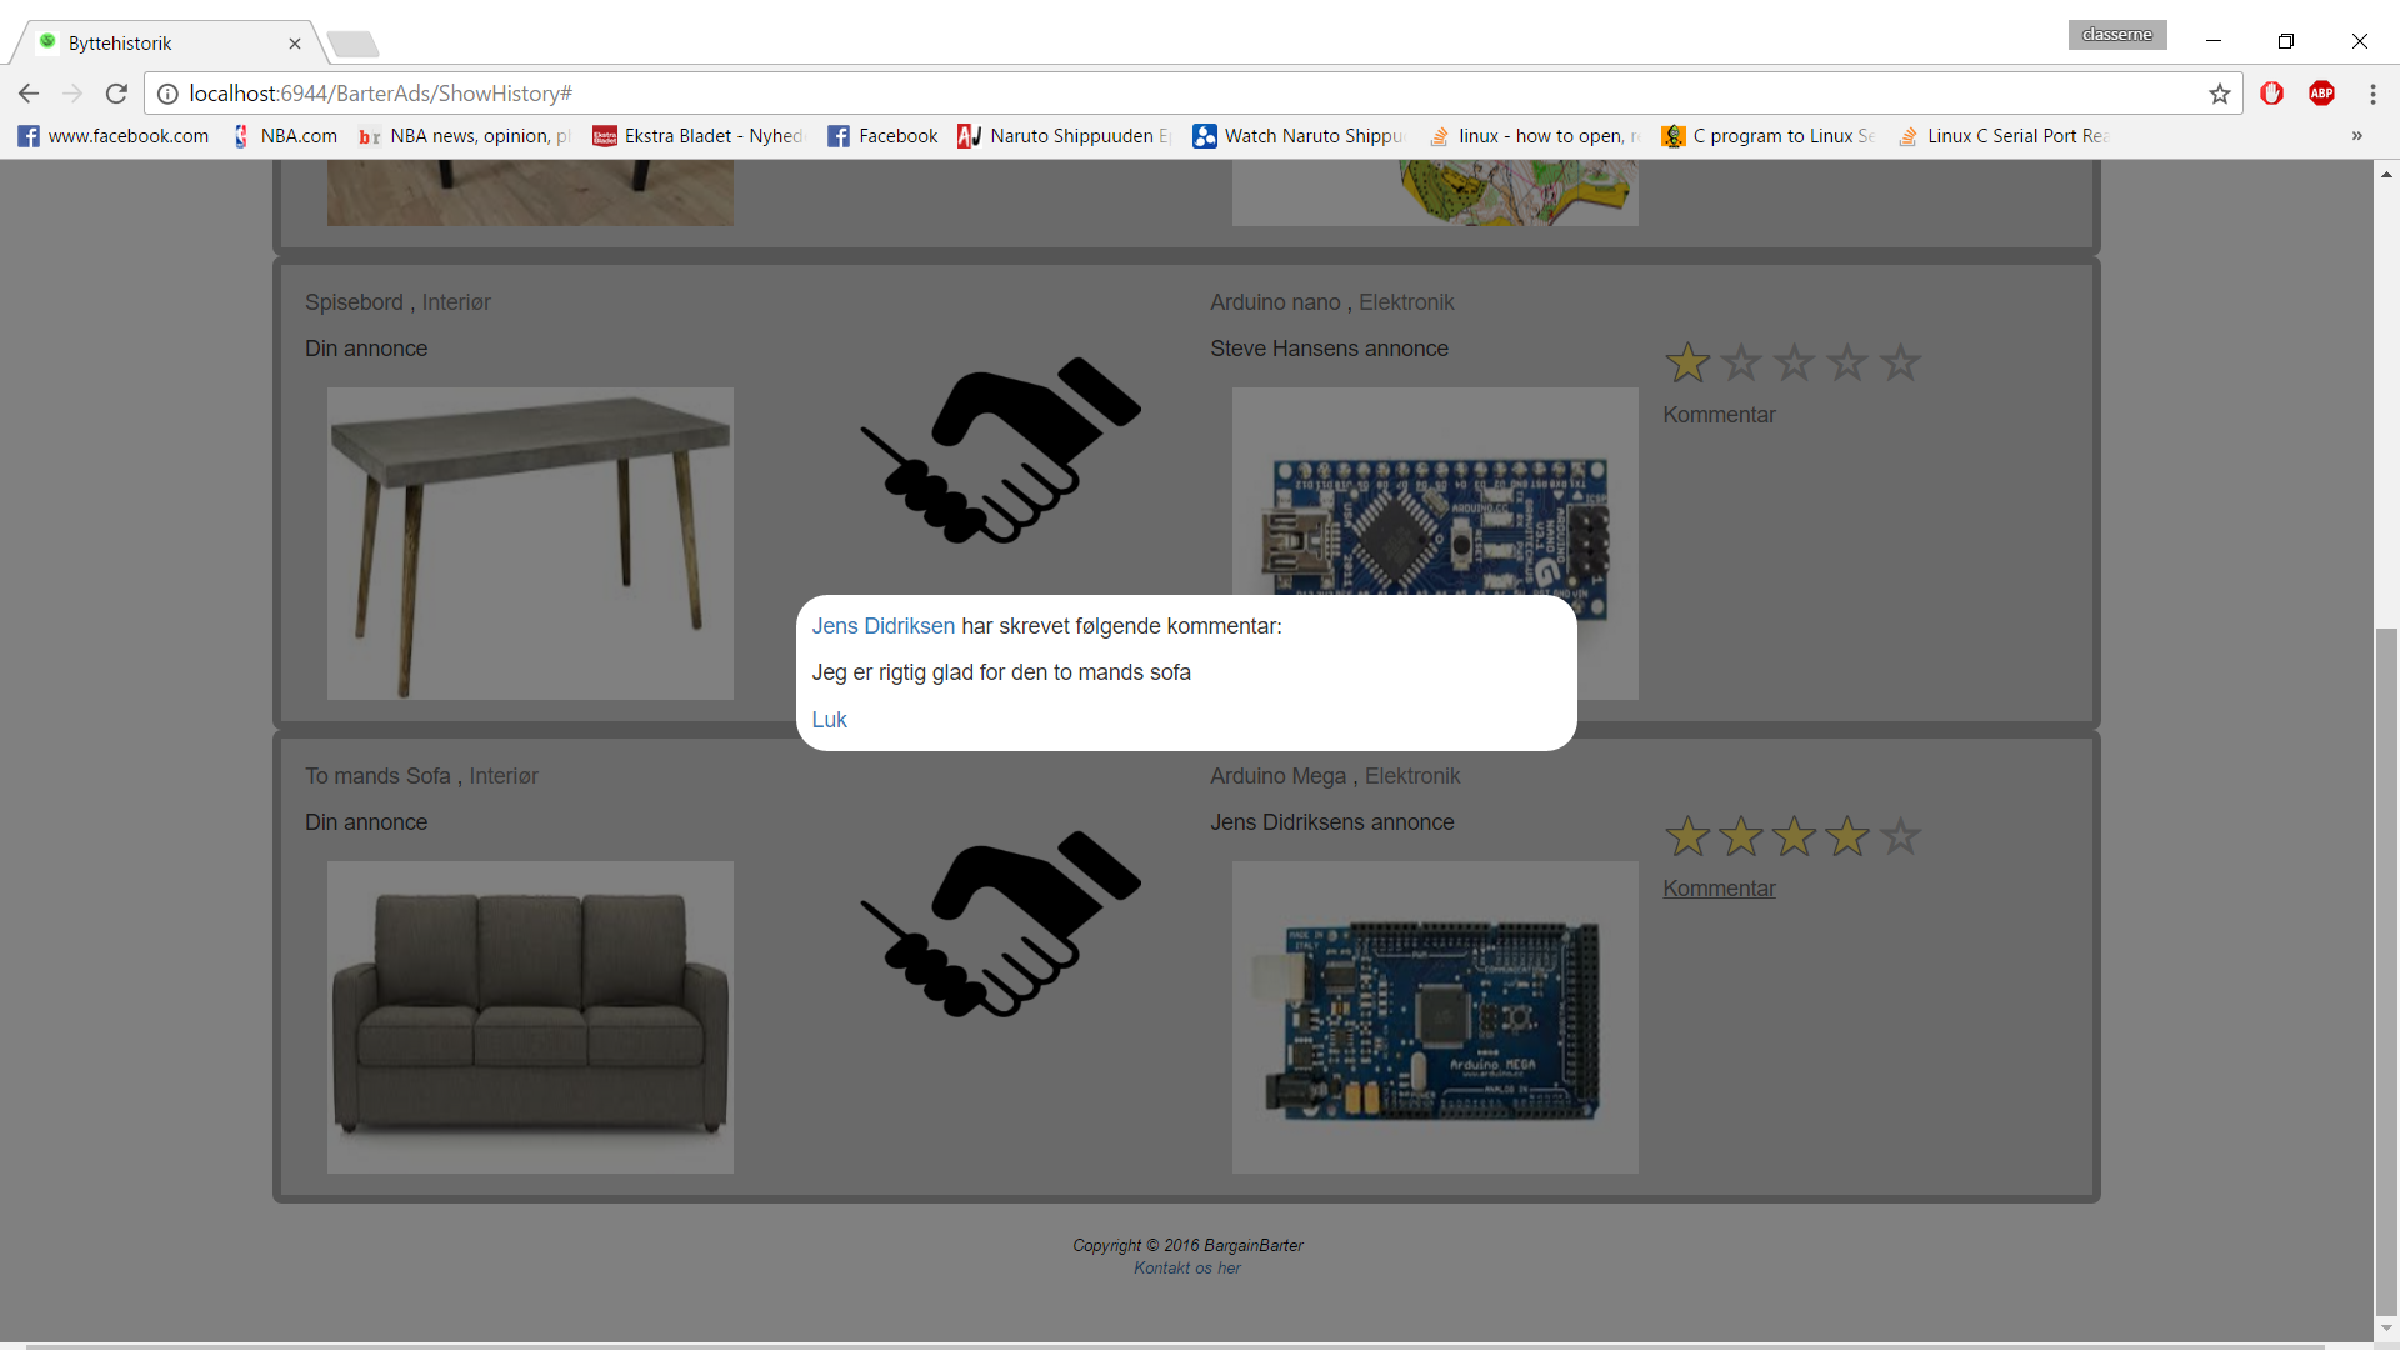
\includegraphics
	[width=165mm]
	{figures/AnmeldtHandel.pdf}
	\caption{Viser rating og popup-kommentar}
	\label{fig:VisKommentar}
\end{figure}




 